%% abtex2-modelo-artigo.tex, v-1.9.7 laurocesar
%% Copyright 2012-2018 by abnTeX2 group at http://www.abntex.net.br/
%%
%% This work may be distributed and/or modified under the
%% conditions of the LaTeX Project Public License, either version 1.3
%% of this license or (at your option) any later version.
%% The latest version of this license is in
%%   http://www.latex-project.org/lppl.txt
%% and version 1.3 or later is part of all distributions of LaTeX
%% version 2005/12/01 or later.
%%
%% This work has the LPPL maintenance status `maintained'.
%%
%% The Current Maintainer of this work is the abnTeX2 team, led
%% by Lauro César Araujo. Further information are available on
%% http://www.abntex.net.br/
%%
%% This work consists of the files abntex2-modelo-artigo.tex and
%% abntex2-modelo-references.bib
%%

% -----
% Versão adaptada para ENCITA
% Autoria Filipe Verri <verri@ita.br>
% Data 22/12/2021
% -----

% ------------------------------------------------------------------------
% ------------------------------------------------------------------------
% abnTeX2: Modelo de Artigo Acadêmico em conformidade com
% ABNT NBR 6022:2018: Informação e documentação - Artigo em publicação
% periódica científica - Apresentação
% ------------------------------------------------------------------------
% ------------------------------------------------------------------------

\documentclass[
	% -- opções da classe memoir --
	article,			% indica que é um artigo acadêmico
	10pt,				% tamanho da fonte
	oneside,			% para impressão apenas no recto. Oposto a twoside
	a4paper,			% tamanho do papel.
  twocolumn,			% para coluna dupla
	english,			% idioma adicional para hifenização
	brazil,				% o último idioma é o principal do documento
	sumario=tradicional,
	]{abntex2}


% ---
% PACOTES
% ---

% ---
% Pacotes fundamentais
% ---
\usepackage{lmodern}			% Usa a fonte Latin Modern
\usepackage[T1]{fontenc}		% Selecao de codigos de fonte.
\usepackage[utf8]{inputenc}		% Codificacao do documento (conversão automática dos acentos)
\usepackage{indentfirst}		% Indenta o primeiro parágrafo de cada seção.
\usepackage{nomencl} 			% Lista de simbolos
\usepackage{color}				% Controle das cores
\usepackage{graphicx}			% Inclusão de gráficos
\usepackage{microtype} 			% para melhorias de justificação
\usepackage{booktabs} % Tabelas
% ---

% ---
% Pacotes de citações
% ---
\usepackage[alf]{abntex2cite}	% Citações padrão ABNT
% ---

% --- Informações de dados para CAPA e FOLHA DE ROSTO ---
\titulo{Caracterização de sistema de propulsão a gás frio com vetorização de empuxo}
\ifthenelse{\equal{\ABNTEXisarticle}{true}}{%
\renewcommand{\maketitlehookb}{}
}{}

\autor{Pedro Kuntz Puglia\thanks{Instituto Tecnológico de Aeronáutica (ITA), pesquisador voluntário,
  \href{mailto:pepuglia@gmail.com}{pepuglia@gmail.com}.},
  Leonardo Gouvêa\thanks{ITA, orientador, gouvea@ita.br}, Maurício Morales\thanks{ITA, co-orientador, morales@ita.br}}

\local{ITA, São José dos Campos, SP, Brasil}
\data{XXVIII Encontro de Iniciação Científica do ITA -- XXVIII ENCITA/2023}
% ---

% ---
% Configurações de aparência do PDF final

% alterando o aspecto da cor azul
\definecolor{blue}{RGB}{41,5,195}

% informações do PDF
\makeatletter
\hypersetup{%pagebackref=true,
		pdftitle={\@title},
		pdfauthor={\@author},
		colorlinks=true,       		% false: boxed links; true: colored links
    	linkcolor=blue,          	% color of internal links
    	citecolor=blue,        		% color of links to bibliography
    	filecolor=magenta,      		% color of file links
		urlcolor=blue,
		bookmarksdepth=4
}
\makeatother
% ---

% ---
% compila o indice
% ---
\makeindex
% ---

% ---
% Altera as margens padrões
% ---
\setlrmarginsandblock{2cm}{2cm}{*}
\setulmarginsandblock{1.5cm}{2.5cm}{*}
\checkandfixthelayout
% ---

% ---
% Espaçamentos entre linhas e parágrafos
% ---

% O tamanho do parágrafo é dado por:
\setlength{\parindent}{0.7cm}

% Controle do espaçamento entre um parágrafo e outro:
\setlength{\parskip}{0.1cm}

% Espaçamento simples
\SingleSpacing

% Espaçamento após título das Referências
\setlength\afterchapskip{\lineskip}

% ----
% Início do documento
% ----
\begin{document}

% Seleciona o idioma do documento (conforme pacotes do babel)
\selectlanguage{brazil}

% Retira espaço extra obsoleto entre as frases.
\frenchspacing

% ----------------------------------------------------------
% ELEMENTOS PRÉ-TEXTUAIS
% ----------------------------------------------------------

% página de titulo principal (obrigatório)
\maketitle

% resumo em português
\begin{resumoumacoluna}
Este trabalho apresenta o processo de desenvolvimento e caracterização de um sistema de vetorização de empuxo com motor a gás frio. O motor tem como requisito empuxo de \(2\;\mathrm{N}\) e \(5\;\mathrm{bar}\) de pressão de câmara. O método de vetorização escolhido para teste foi o de \textit{jet vane}. O motor construído apresentou um impulso específico de \(46,6\;\mathrm{s}\). O sistema foi caracterizado com uma balança de três componentes. Como resultado final, obtiveram-se as derivadas de controle de força lateral e momento. Por fim, apresentaram-se os problemas metodológicos encontrados e \textit{trade-offs} de engenharia identificados para o sistema.
 \vspace{\onelineskip}

 \noindent
 \textbf{Palavras-chave}: propulsão, gás frio, vetorização de empuxo, controle.
\end{resumoumacoluna}
% ---

% ----------------------------------------------------------
% ELEMENTOS TEXTUAIS
% ----------------------------------------------------------
\textual
% ----------------------------------------------------------
% Introdução
% ----------------------------------------------------------
\section{Introdução}

A tecnologia de controle de vetorização de empuxo (ou TVC, do inglês \textit{thrust vector control}) é fundamental para a estabilidade e para o seguimento de trajetória dos foguetes, pois utiliza o direcionamento do empuxo do motor para controlar o veículo. Este trabalho busca iniciar uma linha de pesquisa brasileira sobre o assunto.

O desenvolvimento de sistemas propulsivos é baseado em coeficientes semi-empíricos. O coeficiente de empuxo \(C_F\) e a velocidade característica \(C^*\) podem ser usados para calcular a vazão mássica do motor foguete com~\cite{Sutton}
\begin{equation}
  \label{eq:mass_flow}
  \dot{m} = \frac{F}{C^* C_F}
\end{equation}
ao passo que as áreas das seções transversais da garganta \(A_t\) e da tubeira \(A_e\) podem ser relacionadas pela razão de expansão \(\varepsilon \), dada por
\begin{equation}
  \varepsilon = \frac{A_e}{A_t}\label{eq:exp_ratio}
\end{equation} 

\textit{Jet vanes}, ou lâminas defletoras, consistem em placas imersas no escoamento supersônico à jusante da tubeira do motor foguete. Para pequenas deflexões, escoamento uniforme e espessura infinitesimal, é possível afirmar que a força lateral produzida pelo sistema é proporcional ao ângulo de deflexão~\cite{anderson}. 

A formulação mais usual de controle linear invariante no tempo define uma matriz de controle~\cite{fbsys}, cujas entradas são derivadas de controle, como por exemplo a derivada da força lateral em relação à deflexão da lâmina defletora \(\delta \), dada por
\begin{equation}
  F_{x\delta} = \frac{\mathrm{d} F_x}{\mathrm{d} \delta}\label{eq:control_derivative}
\end{equation}

Sendo assim, este trabalho tem por objetivo final caracterizar as derivadas de controle de um sistema de vetorização de empuxo com um motor foguete de gás frio de pequena escala (\(2\;\mathrm{N}\)), bem como caracterizar seus coeficientes propulsivos e \textit{trade-offs} de engenharia relacionado ao sistema de vetorização de empuxo.

\section{Materiais e métodos}

O sistema propulsivo foi projetado de maneira programática com o auxílio do CEA NASA~\cite{ceanasa} e sua interface programática RocketCEA~\cite{rocketcea}. Foram levantados como requisitos empuxo \(F = 2\;\mathrm{N}\), pressão de câmara \(p_c = 500\;\mathrm{kPa}\), temperatura do propelente \(T_{\mathrm{prop}} = 298,15\;\mathrm{K}\). Estes dados foram inseridos no CEA para cálculo áreas das seções transversais de garganta e tubeira. A área da seção transversal da câmara foi escolhida empiricamente.

O motor a gás frio e o sistema de vetorização foram manufaturados em ABS por impressão 3D. Para as medidas de força em função da deflexão da lâmina, foi utilizada a balança de três componentes Plint \& Partners disponível no Laboratório de Engenharia Aeronáutica. A saída da balança, as forças \(F_A\) (\textit{aft}), \(F_F\) (\textit{fore}) e \(F_D\) (\textit{drag}) em cada extensômetro, pode ser convertida nas forças horizontal \(F_x\), vertical \(F_y\) e no momento atuante \(M\) com o conhecimento da distância \(d\) entre as componentes \textit{aft} e \textit{fore}~\cite{lab}.

\begin{figure}[htbp]
  \centering
  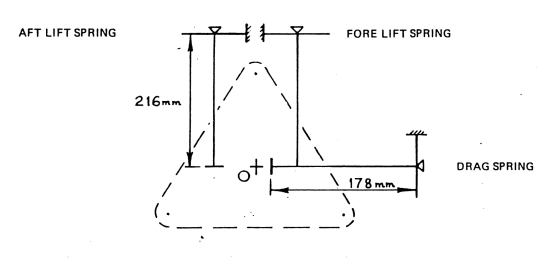
\includegraphics[width=\linewidth]{../report/img/three_axis_scale_diagram.png}
  \caption{Diagrama da balança de três componentes.}\label{fig:diag_three_axis_scale}
\end{figure}

\section{Resultados e Discussão}

Obtiveram-se empiricamente para o motor \(\varepsilon = 1,35\), \(C^* = (368,8 \pm 2,4)\;\mathrm{m}\;\mathrm{s}^{-1}\) e \(C_{F} = 1,228 \pm 0,005\), constituindo uma vazão mássica de \(\dot{m} = (4,42 \pm 0,03)\;\mathrm{g}\;\mathrm{s}^{-1}\). Obteve-se portanto um impulso específico de \(46,6\;\mathrm{s}\). A alta vazão mássica e o baixo impulso específico devem-se ao baixo conteúdo energético do ar comprimido usado no experimento. 

O motor desenvolvido, montado no sistema de vetorização de empuxo, pode ser visto na Fig.~\ref{fig:assembled_system}. A lâmina é movimentada pelo servomotor à direita da figura, podendo atingir deflexões de \(\pm 20\mathrm{^\circ}\). 

\begin{figure}[htbp]
  \centering
  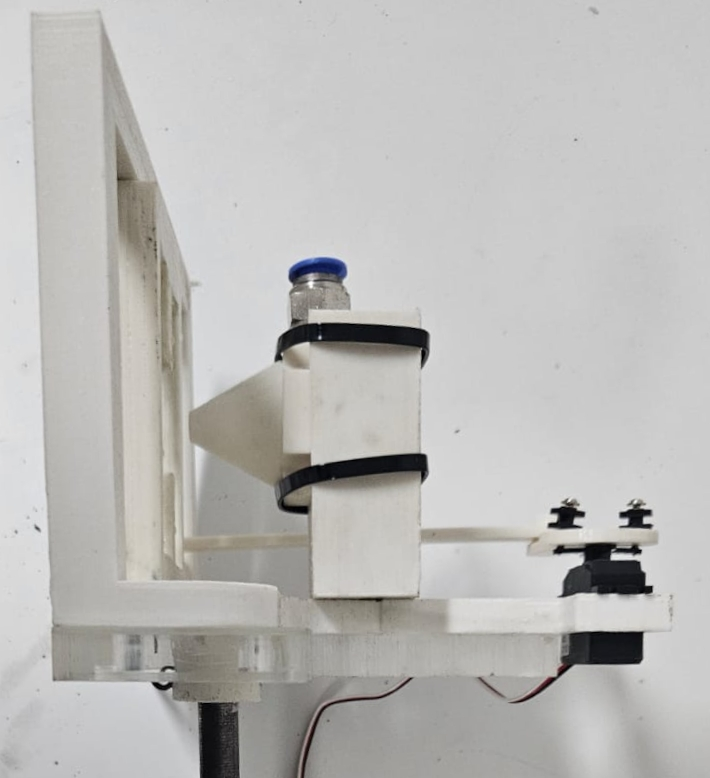
\includegraphics[width=.7\linewidth]{../report/img/tvc_assembly_right_cropped.jpeg}
  \caption{Montagem do sistema de vetorização de empuxo.}\label{fig:assembled_system}
\end{figure}

Na Figura~\ref{fig:data} observam-se as curvas de \(F_y\), paralela ao empuxo, \(F_x\), força lateral causada pelo sistema, e \(M\), momento em relação ao eixo da balança. Observa-se que a posição \(90\;\mathrm{^\circ}\) corresponde à lâmina não defletida. Devido à simetria da geometria, nesta posição seria esperado haver força lateral e momento nulos, o que não ocorreu empiricamente devido à presença da mangueira de alimentação de ar conectada ao motor. Observam-se também flutuações no valor do empuxo, devidos possivelmente ao esvaziamento do reservatório do compressor de ar. Este fenômeno é favorecido pela alta vazão mássica exigida.

Apesar dos problemas descritos, foi possível validar um grande número de hipóteses uteis para aplicações de controle. Por exemplo, verifica-se na Fig.~\ref{fig:data} a linearidade das forças produzidas até aproximadamente \(15\;\mathrm{^\circ}\) de deflexão, o que permite o cálculo das derivadas de controle em relação ao eixo da balança como \(F_{x\delta} = (3,57 \pm 0,05)\times10^{-2} \mathrm{N} / \mathrm{^\circ}\) e \(M_\delta = (-2,29 \pm 0,02)\times10^{-2} \mathrm{N}\;\mathrm{cm} / \mathrm{^\circ}\).

\begin{figure}[htbp]
  \centering
  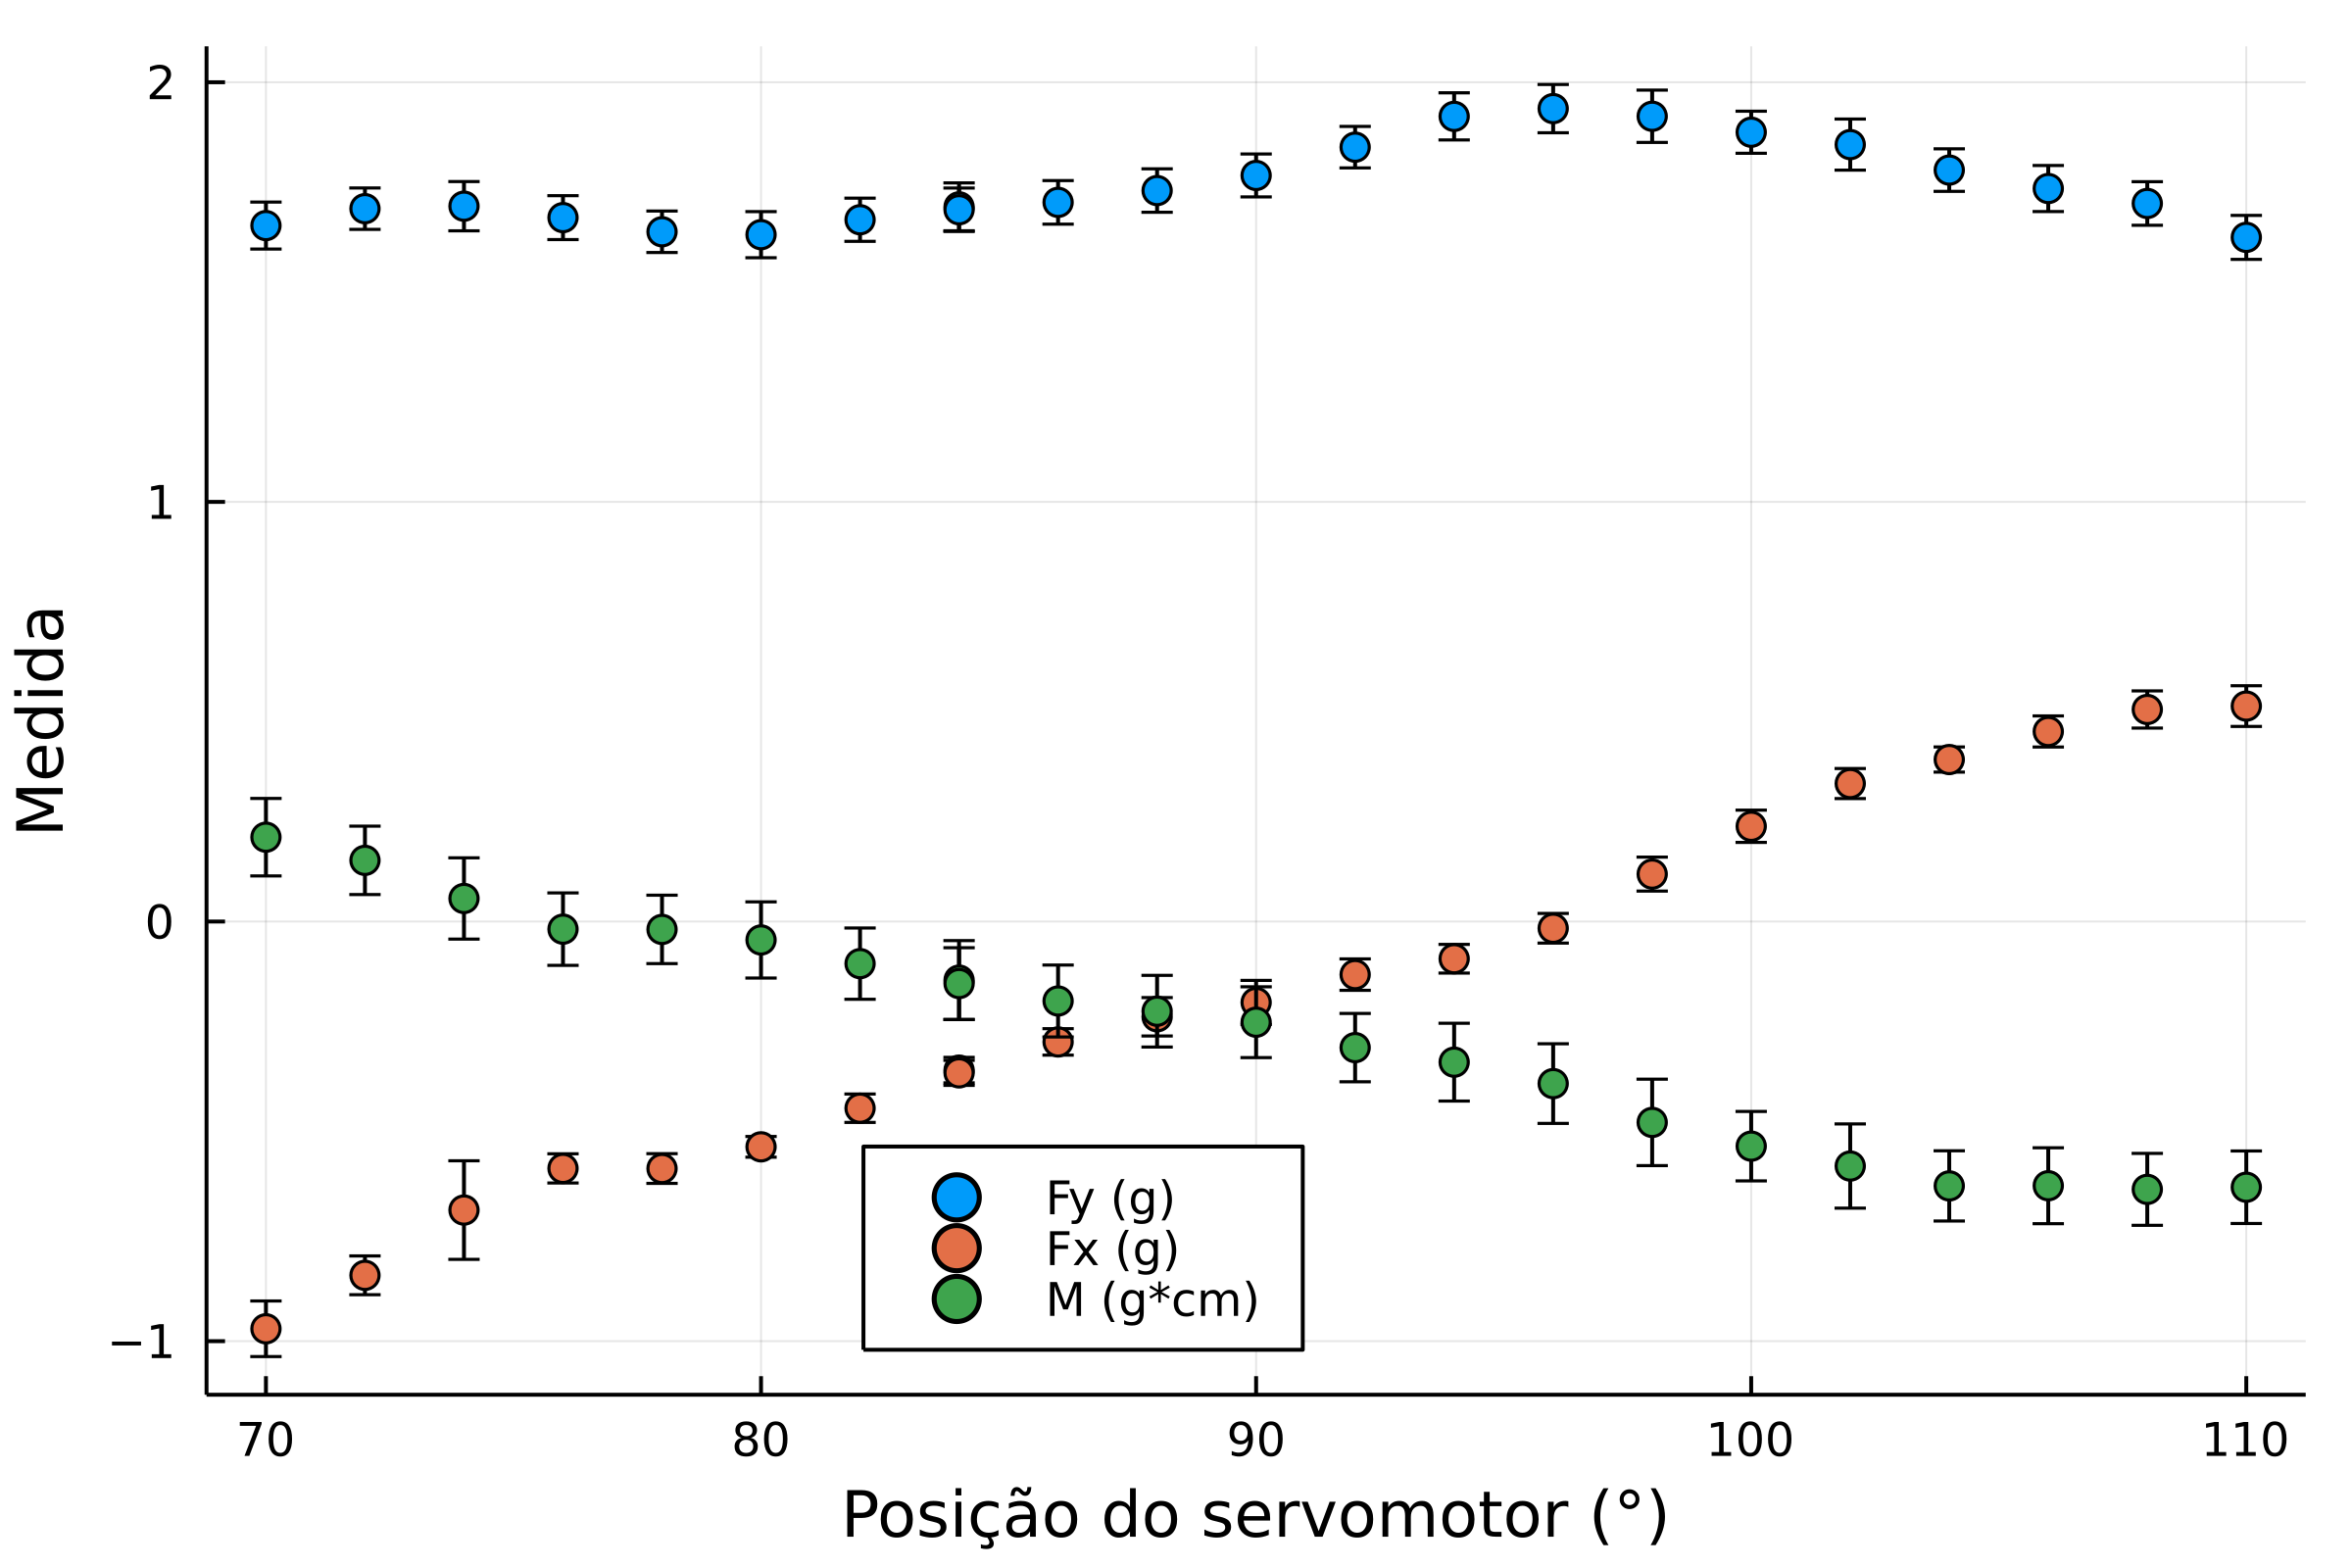
\includegraphics[width=.7\linewidth]{../report/img/results/exp10_5bar_110_a_70.png}
  \caption{Dados experimentais de forças e momento em função da deflexão da lâmina defletora.}\label{fig:data}
\end{figure}

Por fim, foram identificados \textit{trade-offs} de engenharia associados ao sistema. Citam-se, por exemplo, a espessura da lâmina, que afeta o arrasto de onda gerado~\cite{anderson}, reduzindo a eficiência, bem como a distância da tubeira à lâmina, que afeta as derivadas de controle do sistema.

\section{Conclusões e Recomendações}

A proposta deste trabalho, de desenvolver um sistema de vetorização de empuxo e caracterizar seu desempenho, foi executada. Desenvolveu-se um istema de vetorização de empuxo com lâmina defletora de gás frio de \(2\;\mathrm{N} \). Este sistema foi caracterizado em relação à perda de empuxo causada pela adição da lâmina defletora e suas derivadas de controle foram obtidas. Apesar do objetivo ter sido atingido, foram encontradas várias dificuldades e fontes de erros experimentais que devem ser abordadas em trabalhos futuros.

\section{Agradecimentos}

Ao professor Leonardo Gouvea pela oportunidade, ao professor Tiago Barbosa por disponibilizar a balança, e aos técnicos Wilson e Newton por sua dedicação, bem como ao João Baldo e Arthur Zoppi pelo auxílio com as impressões 3D.
% ----------------------------------------------------------
% Referências bibliográficas
% ----------------------------------------------------------
\bibliography{artigo-encita}

\end{document}
